\documentclass[titlepage]{article}
\usepackage{graphicx}
\usepackage{amsmath}

\begin{document}

\title{Experiment 1: Uniform Acceleration}
\author{Tian Ye \\ \\ UID: 704931660 \\ \\ TA: Wen Li Wen \\ \\ Lab Partner: Matthew Barba \\ \\ Lab 8 Tuesday 6:00 PM}
\date{October 10th, 2017}

\maketitle

\section{Introduction}
Experiment 1 centers about finding the magnitude of acceleration as gravity acts on a mass that is strung over a pulley, which in turn pulls a glider that is suspended over a nearly frictionless track.

\subsection{Solving for Acceleration}
To solve for acceleration of the glider, we first create free body diagrams for both the glider and the mass. The diagrams for both are displayed below:

\begin{figure}[!htbp]
    \centering
    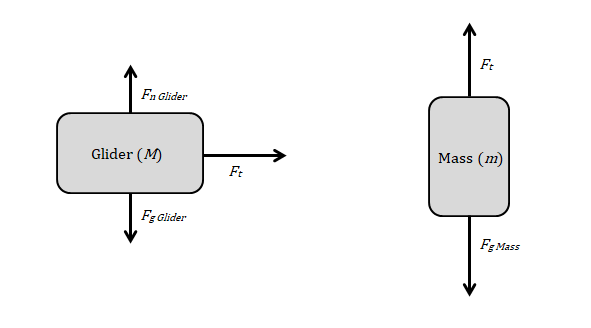
\includegraphics[width=4.0in]{FreeBody.png}
    \caption{Free body diagrams for both the glider and the mass. Note that while steps were taken to minimize friction in the experiment, it is still present nonetheless. However, it was omitted from the diagram since its effect is negligible in this case.}
\end{figure}

From the diagram we can see that $\Sigma F$ on the mass is the difference between the force of gravity, $F\textsubscript{g Mass}$ which is given by $mg$, and the tension force, $F\textsubscript{t}$. Similarly, for the glider we can see that $\Sigma F$ is just the tension force $F\textsubscript{t}$ since $F\textsubscript{g Glider}$ and $F\textsubscript{n Glider}$ cancel each other out as they are equal in magnitude and opposite in direction. Using the known relationship that $\Sigma F=ma$, we can find the following:

\begin{equation}
\begin{split}
 F\textsubscript{t} &= Ma\\
ma &= mg - F\textsubscript{t} \\
&= mg - Ma \\
a &= \frac{mg}{m+M}
\end{split}
\end{equation}

With m and M referring to the masses of the mass and glider, respectively. 

\subsection{Solving for Uncertainty of Acceleration}
Next, we need to find $\delta a$, using Equation ii.14 from the lab manual. Taking the partial derivative of a in terms of both m and M, we find the following:

\begin{align*}
\delta a\textsubscript{m} &= \frac{\partial a}{\partial m}\delta m & \delta a\textsubscript{M} &= \frac{\partial a}{\partial M}\delta M\\
&= \frac{Mg}{(m+M)^2}\delta m & &=-\frac{mg}{(m+M)^2}\delta M
\end{align*}

From this, we can derive the total uncertainty of $a$ from using again Equation ii.14:

\begin{equation}
\begin{split}
\delta a &= \sqrt{\delta a^2\textsubscript{m}+\delta a^2\textsubscript{M}} \\
&= \sqrt{\bigg (\frac{Mg}{(m+M)^2}\delta m\bigg )^2 + \bigg (-\frac{mg}{(m+M)^2}\delta M \bigg )^2} \\
&= \frac{g}{(m+M)^2}\sqrt{(M\delta m)^2 + (-m\delta M)^2}
\end{split}
\end{equation}

\section{Data Analysis}
There are two methods to find acceleration: predicted acceleration via equations and measured acceleration via the collected data points.

\subsection{Predicted Acceleration}
To find our predicted acceleration, we will use Equation 1, derived earlier, to find our acceleration using the measured values for mass of the glider and various hanging weights.

\begin{table}[!htbp]
\renewcommand{\arraystretch}{1.3}
\centering
\begin{tabular}{c|c}
    \hline
    \hline
    Mass of Weight &  Uncertainty\\
    \hline
    \hline

    2.5 grams     &  $\pm$ 0.5 grams \\
    \hline

    5.5 grams    &   $\pm$ 0.5 grams \\
    \hline

    10 grams  &  $\pm$ 1 gram\\
    \hline

    19.5 grams  &  $\pm$ 1.5 grams\\
    \hline

    22 grams  &  $\pm$ 2 grams\\
    \hline
    \hline
    \hline
    Mass of Glider & Uncertainty\\
    \hline
    \hline

    224 grams & $\pm$ 2 grams\\
    \hline
\end{tabular}
\caption{The masses and their corresponding uncertainties that were used for this experiment. Mass was determined via balancing scale.}
\end{table}

\pagebreak

Plugging our values into Equation 1 and Equation 2 for acceleration and uncertainty of acceleration, respectively, we are presented with the following results:

\begin{table}[!htbp]
\renewcommand{\arraystretch}{1.3}
\centering
\begin{tabular}{c|c}
    \hline
    \hline
    Mass of Hanging Weight (kg) &  Predicted Acceleration (m/s$^2$)\\
    \hline
    \hline

    0.0025 $\pm$ 0.0005 &  0.108 $\pm$ 0.021 \\
    \hline

    0.0055 $\pm$ 0.0005 &  0.235 $\pm$ 0.021 \\
    \hline

    0.010 $\pm$ 0.001 &  0.419 $\pm$ 0.040 \\
    \hline

    0.0195 $\pm$ 0.0015 &  0.785 $\pm$ 0.056 \\
    \hline

    0.022 $\pm$ 0.002 &  0.876 $\pm$ 0.073 \\
    \hline
\end{tabular}
\caption{Measured mass of weights in kilograms used in calculations with their respective uncertainties and their respective predicted acclerations with their respective uncertainties. Values were obtained by using Equation 1 and Equation 2}
\end{table}

\pagebreak

\subsection{Measured Acceleration}
To find our measured acceleration, we will use the data points collected earlier in the lab. 

\subsubsection{Lab Setup}
The data was collected by rotating a ''smart pulley'' that recorded the time at which each full revolution occurred. The pulley is rotated by a string that connects the mass to the glider, as shown in the figure below:

\begin{figure}[ht]
    \centering
    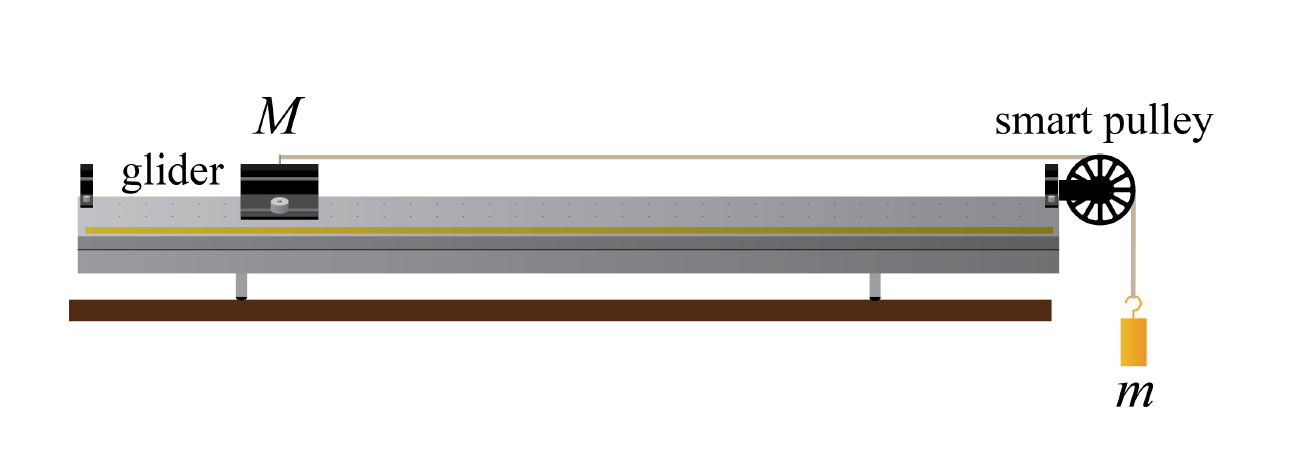
\includegraphics[width=4.0in]{Diagram.png}
    \caption{Visual representation of the glider, pulley, and mass system. Figure reproduced
(with permission) from Fig. 1.1 by Campbell, W. C. \textit{et al.\textsuperscript{1}}.}
\end{figure}

\subsubsection{Data Collection}
When the mass is dropped, the string that is pulling the glider also rotated the smart pulley, which then recorded two sets of data: the ''blocks'', or number of revolutions made by the pulley, and the time at which each block was measured. 

\subsubsection{Calculation and Analysis}
In order to solve for velocity, and subsequently, acceleration from this data set, we had to first use the given constant $\kappa = (1.50 \pm 0.05)$ cm/block to solve for the displacement of the glider by multiplying the block number by $\kappa$ . We ignore $\delta\kappa$ as it is statistical uncertainty, and consequently is reflected in the spread of the data points. Afterwards, to solve for velocity between each time interval, the following equation was used:

\[
\bar v = \frac{x\textsubscript{i+1}-x\textsubscript{i}}{t\textsubscript{i+1}-t\textsubscript{i}}
\]

Where $x\textsubscript{i}$ refers to displacement obtained by multiplying block number by $\kappa$, and $t\textsubscript{i}$ refers to change in time interval between each block measurement.

To solve for time interval, we averaged the time interval between each value, which also in turn gave us the same number of time data points as velocity:

\[
\bar t = \frac{t\textsubscript{i+1}+t\textsubscript{i}}{2}
\]

By plotting $\bar v$ against $\bar t$ in Microsoft Excel, we were able to find the approximate acceleration of the glider as $a = \frac{\Delta v}{\Delta t}$ \\

Therefore the slope of the best fit lines generated by Microsoft Excel will be an estimate of the true acceleration of the glider for the various masses.

\begin{figure}[ht]
    \centering
    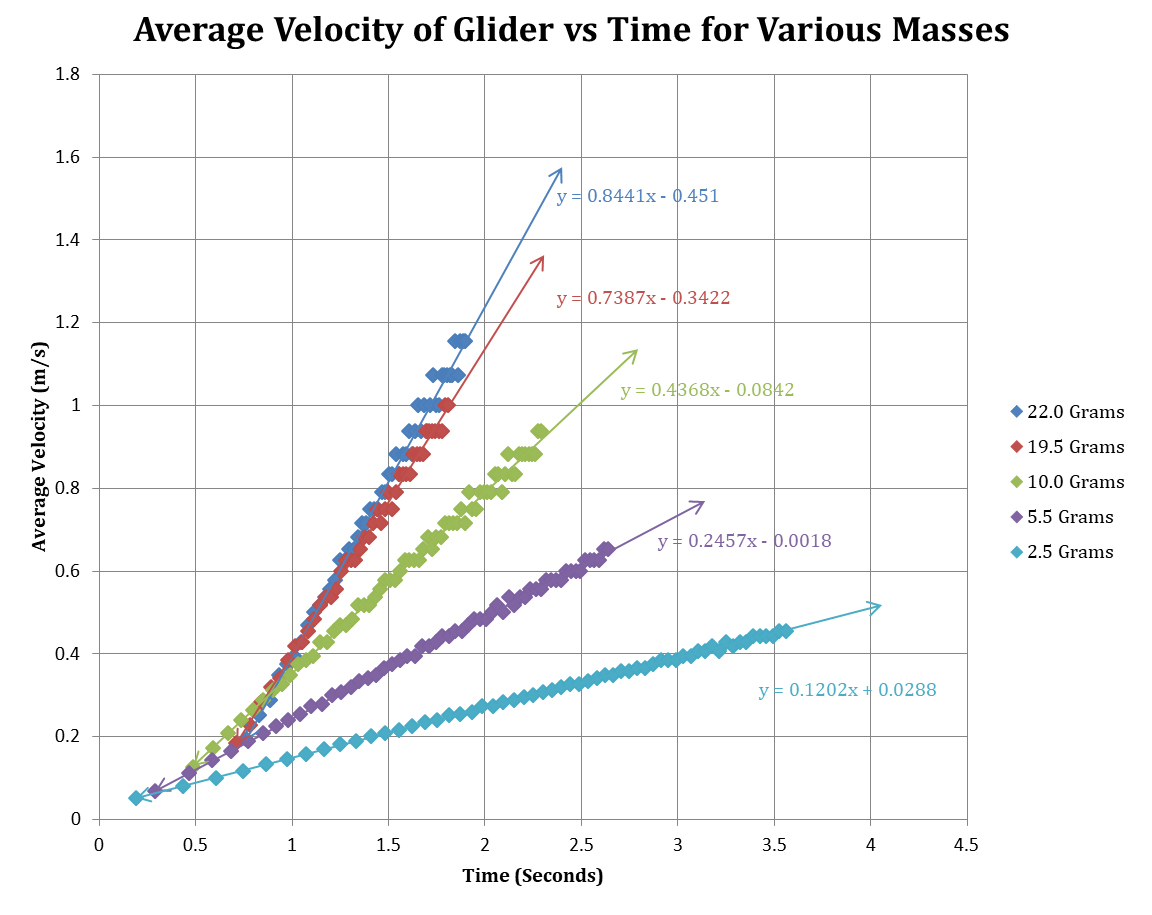
\includegraphics[width=5.0in]{Graph.png}
    \caption{Velocity vs Time graph of the glider for various masses. Each mass has its own color for its linear fit line, equation, and data points. The same glider was used for all tests. The slope of these lines represents the measured acceleration.}
\end{figure}

\pagebreak

To solve for uncertainty of each slope, we then use Microsoft Excel's data analysis function; the results of which for each mass are recorded in the table below:

\begin{table}[!htbp]
\renewcommand{\arraystretch}{1.3}
\centering
\begin{tabular}{c|c}
    \hline
    \hline
    Mass of Hanging Weight (kg) &  Measured Acceleration (m/s$^2$)\\
    \hline
    \hline

    0.0025 $\pm$ 0.0005 &  0.1202 $\pm$ 0.0004 \\
    \hline

    0.0055 $\pm$ 0.0005 &  0.246 $\pm$ 0.001 \\
    \hline

    0.010 $\pm$ 0.001 &  0.437 $\pm$ 0.004 \\
    \hline

    0.0195 $\pm$ 0.0015 &  0.739 $\pm$ 0.007 \\
    \hline

    0.022 $\pm$ 0.002 &  0.84 $\pm$ 0.01 \\
    \hline
\end{tabular}
\caption{Measured mass of weights in kilograms used in Excel with their respective uncertainties and their respective measured acclerations with their respective uncertainties. The same glider was used for all tests. Values were obtained by using the Regression tool in Microsoft Excel}
\end{table}

\pagebreak

\section{Conclusion}
The goal of Experiment 1 was to find several different accelerations of a glider as it was pulled along a frictionless track by a mass that is connected to the glider and hanging over a pulley. The results for the experiment were reached via two different methods: via calculating acceleration via equations and free body diagrams or by solving for measured velocity and time and plotting them against one another in order to obtain the slope. A table listing all the results is shown below:


\begin{table}[!htbp]
\renewcommand{\arraystretch}{1.3}
\centering
\scalebox{0.7}{
\begin{tabular}{c|c|c}
    \hline
    \hline
    Mass of Hanging Weight (kg) &  Predicted Acceleration (m/s$^2$) & Measured Acceleration (m/s$^2$)\\
    \hline
    \hline

    0.0025 $\pm$ 0.0005 &  0.108 $\pm$ 0.021 &  0.1202 $\pm$ 0.0004 \\
    \hline

    0.0055 $\pm$ 0.0005 &  0.235 $\pm$ 0.021 &  0.246 $\pm$ 0.001 \\
    \hline

    0.010 $\pm$ 0.001 &  0.419 $\pm$ 0.040 &  0.437 $\pm$ 0.004 \\
    \hline

    0.0195 $\pm$ 0.0015 &  0.785 $\pm$ 0.056 &  0.739 $\pm$ 0.007 \\ 
    \hline

    0.022 $\pm$ 0.002 &  0.876 $\pm$ 0.073 &  0.84 $\pm$ 0.01 \\
    \hline
\end{tabular}
}
\caption{Combined data for Table 2 and Table 3}
\end{table}

The reason for the discrepancy between the predicted acceleration and measured acceleration can be attributed to various sources of error, the most notable of which being friction. Neither air resistance nor kinetic friction were accounted for in the free body diagrams and the calculations associated with them. \\
Another source of error that most likely explains why the predicted acceleration is lower in magnitude than the measured acceleration for certain data values is that the track is not perfectly level. Any object of substantial length bends downward slightly under its own weight. As the track was not positioned nearly high enough above the ground so that the mass would accelerate the glider for the entire length, but rather for only approximately 3/4 of the length, the glider would have been traveling primarily down the part of the track that curves slightly downwards, causing the glider to also be accelerated by a component of gravity as well. \\
Finally, the fact that neither the string nor the pulley are ideal could also have led some error in the data measurement, such as the larger spread of data as the velocity increased over time.

\pagebreak

\section{Extra Credit}

For this particular analysis, the 2.5 gram test data was used as it was the most linear of all the data.

\begin{figure}[ht]
    \centering
    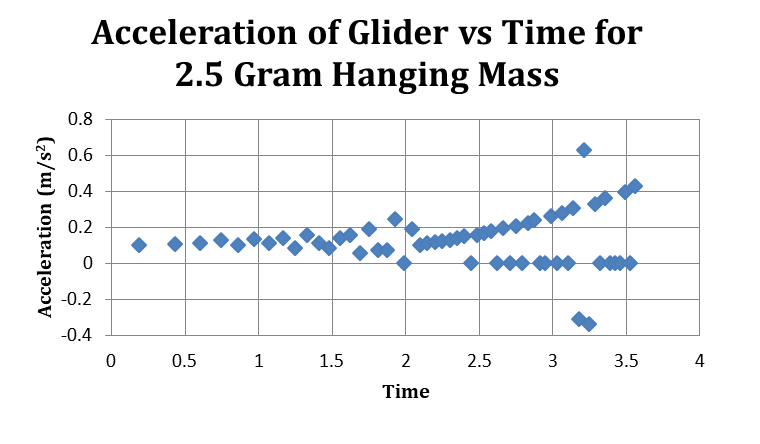
\includegraphics[width=3.5in]{ExtraCredit.png}
    \caption{Acceleration vs Time graph of the glider for 2.5 gram mass.}
\end{figure}

\subsection{Analysis}
A quick glance at the graph of acceleration plotted against time shows that while the data begins relatively constant, it quickly begins to fluctuate significantly around the 2 second mark, the fluctuation increasing drastically as it approaches the end of the recorded data. 

There is a small fluctuation initially, which is to be expected, and the acceleration is relatively constant since as shown in Equation 1, the acceleration is dependent on nonvariable constants $g$, $m$, and $M$. However, at around the two second mark, the acceleration begins to deviate. This is due to the manner in which the data is recorded.

The "smart pulley" records data as number of revolutions completed and the point of time at which said revolution occurred. Thus, as velocity increases, the time frame between each "block" decreases rapidly, and thus even small deviations and inconsistencies are magnified significantly when the derivative of the positional data is taken twice. By taking $\frac{\Delta x}{\Delta t}$ and subsequently $\frac{\Delta v}{\Delta t}$, we are in essence using Reimann sums to calculate acceleration.

One possible source of inconsistency is the fact that air resistance is a frictional force proportional to velocity. Consequently, as velocity increases, the force of air resistance against the acceleration due to tension in the string can be thought of as a form of oscillation, with the force of air resistance slowing the glider down until the force of tension is greater, whereby the glider is then accelerated forward again.

\subsection{Conclusion}
When the acceleration data is averaged, we find that $\bar a = 0.12$ m/s$^2$ and that the sample standard deviation is 0.15, with a standard error of $\pm$ 0.02. Comparing these values to the measured acceleration, we find that the while both values for acceleration are similar, the standard error of this method,  $\pm$ 0.02, is significantly greater than the standard error of the measured acceleration, \\ $\pm$ 0.0004. Therefore, it can be concluded that generally, it is more accurate to calculate acceleration via fitting a linear fit line to a velocity vs time graph than by differentiating the data a second time.

\pagebreak

\section{Bibliography}

[1] Campbell, W. C. \textit{et al}. Physics 4AL: Mechanics Lab Manual (ver. April 3, 2017).
(Univ. California Los Angeles, Los Angeles, California).

\end{document}
T